\chapter*{Appendix A: User Manual}
The executable versions of the program (together with an example asset file) could be found in the `executables' folder in project submission.

\begin{itemize}
  \item To start the program on \textbf{Windows}, open the folder in the folder `executables' containing the file `portOptWin.exe' and the example data file `assetTest.txt', and simply double click on the executable file.
  \item To run the program on \textbf{Unix/Linux}, open a terminal in the folder `executables' containing the executable file `portfOptUnix'. Make sure that the complied Haskell program `portfOptUnix' and the asset file (`assetTest.txt' for example) are in the same folder. To start the program, simply type into the terminal ``./portfOptUnix'' without the double quotes.
\end{itemize}

After starting the program you are asked to enter the name of the file containing the portfolio information. Make sure the file name does not contain any space and that the file extension is correct. If the file does have spaces, replace them with an underscore, example ``file with spaces.txt'' should be changed to ``file\_with\_spaces.txt''. This is just a precaution so the system does not get confused. Figure~\ref{fig:asset_file} shows what you should see. 
\begin{figure}[H]
  \centering
    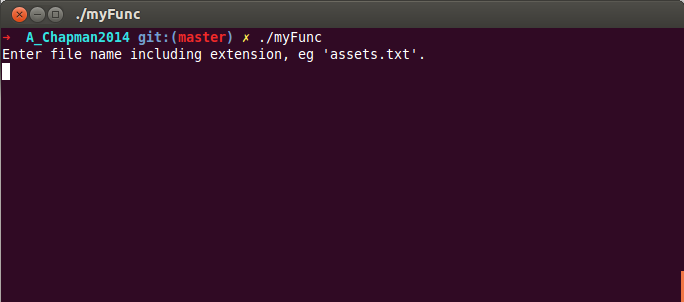
\includegraphics[width=0.9\textwidth]{asset_file}
  \caption{Enter file.}
  \label{fig:asset_file}
\end{figure}
After entering the correct name of the file, you will be asked to type in the number of particles for the swarm in PSO, no more than 50 is needed. Figure~\ref{fig:np} shows what you should see. 
\begin{figure}[H]
  \centering
    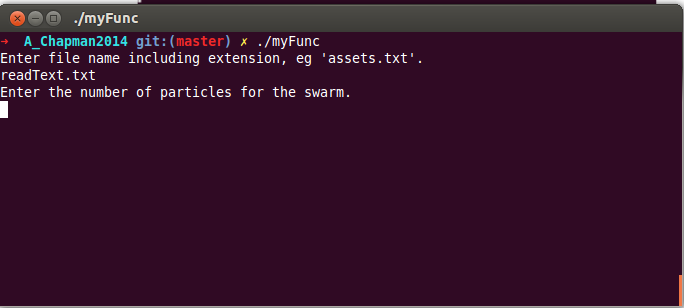
\includegraphics[width=0.9\textwidth]{np}
  \caption{Enter the number of particles}
  \label{fig:np}
\end{figure}
Then you will be asked to enter the number of iterations for the PSO to run for. Figure~\ref{fig:nit} shows what you should see. 
\begin{figure}[H]
  \centering
    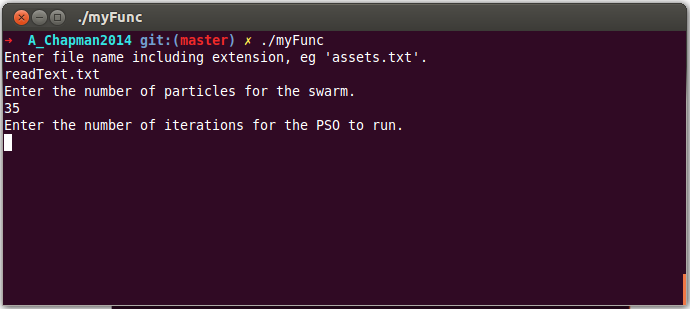
\includegraphics[width=0.9\textwidth]{nit}
  \caption{Enter number of iterations}
  \label{fig:nit}
\end{figure}
Followed the level of risk, 0.5 is neutral. Figure~\ref{fig:risk} shows what you should see. 
\begin{figure}[H]
  \centering
    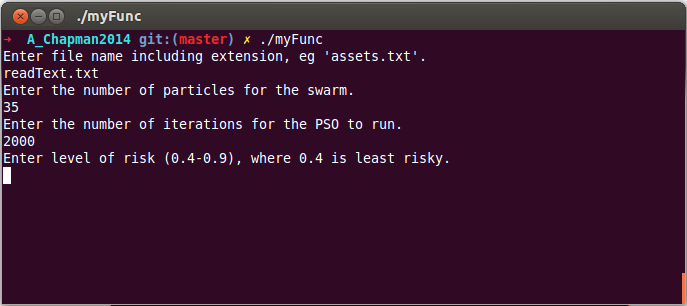
\includegraphics[width=0.9\textwidth]{risk}
  \caption{Enter level of risk}
  \label{fig:risk}
\end{figure}
Then input the lever of risk aversion, recommended is 3. Figure~\ref{fig:aversion} shows what you should see. 
\begin{figure}[H]
  \centering
    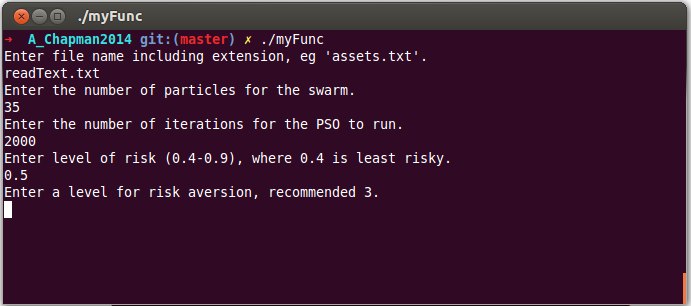
\includegraphics[width=0.9\textwidth]{aversion}
  \caption{Enter level of risk aversion}
  \label{fig:aversion}
\end{figure}
Finally, your expected required portfolio return. Figure~\ref{fig:portReq} shows what you should see. 
\begin{figure}[H]
  \centering
    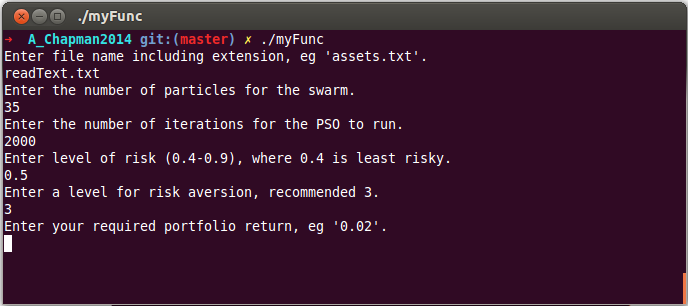
\includegraphics[width=0.9\textwidth]{portReq}
  \caption{Enter expected required return}
  \label{fig:portReq}
\end{figure} 
PSO is pretty quick so you will, if nothing was wrongly inputted, get an answer almost instantaneously. The system will display the ``un-prettified''results on the window. Figure~\ref{fig:results} shows what you should see. 
\begin{figure}[H]
  \centering
    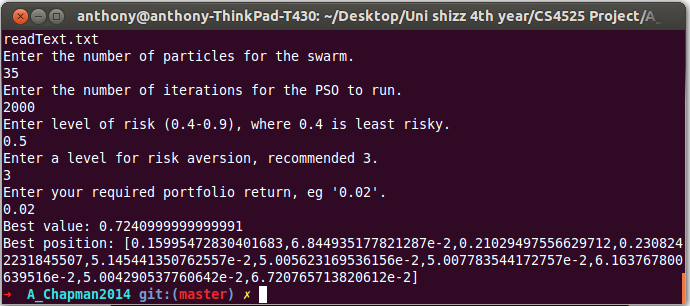
\includegraphics[width=0.9\textwidth]{results}
  \caption{Displaying results on command line}
  \label{fig:results}
\end{figure}
For the better looking results, open the folder containing the output file. The name will be ``output-(date).txt'' for example, output-(2014,5,1).txt. It will contain a file with the proportions of the optimal portfolio. Figure~\ref{fig:output} shows what you should see, where it states that you should invest 11.37\% on asset \textit{Aa}, 5.35\% on asset \textit{Bb}, and so on. 
\begin{figure}[H]
  \centering
    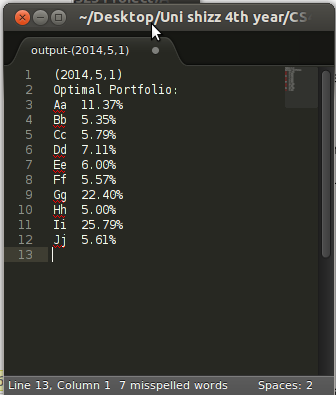
\includegraphics[width=0.9\textwidth]{output}
  \caption{Example output file.}
  \label{fig:output}
\end{figure}
